\section{Confidence Intervals} \todo{section needs a lot of work}

Confidence Intervals are used to convey the uncertainty in a measurement.  For example, if the distance from point A to point B is measured infinite times with a mean of $\overline{AB} = 10.00m$ and a standard deviation of $\sigma_{\overline{AB}}= 0.10m$. This measurement could be written as $\overline{AB} = 10.00m \pm 0.10m$.  Based on this information, each of the following statements is an accurate confidence interval:
\begin{itemize}
	\item The true value of the distance $\overline{AB}$ is expected to lie between 9.90 and 10.10 68.2\% of the time
	\item The true value of the distance $\overline{AB}$ is expected to lie between 9.80 and 10.20, 95.4\% of the time.
	\item The true value of the distance $\overline{AB}$ is expected to lie between 9.60 and 10.40, 99.9937\% of the time.
\end{itemize}

*Note: I'm not really sure if confidence intervals are open or closed... and I'm not sure it matters since the odds that value will be a finite number is 0\%.  In other words, the odds of the true value lying on the edge of a confidence interval is so low that it really shouldn't matter.

The previous example is comparing the mean of an observation, the confidence interval is governed by the t-distribution.  The t-distribution is based on the degrees of freedom, which in this case we defined as being infinitely large.  When the degrees of freedom are infinite, the t distribution is equivalent to the normal distribution.  As the degrees of freedom become smaller, the confidence in the mean and standard deviation get worse, and therefore the confidence interval increases, as shown below.  

\begin{figure}[H]
	\centering
	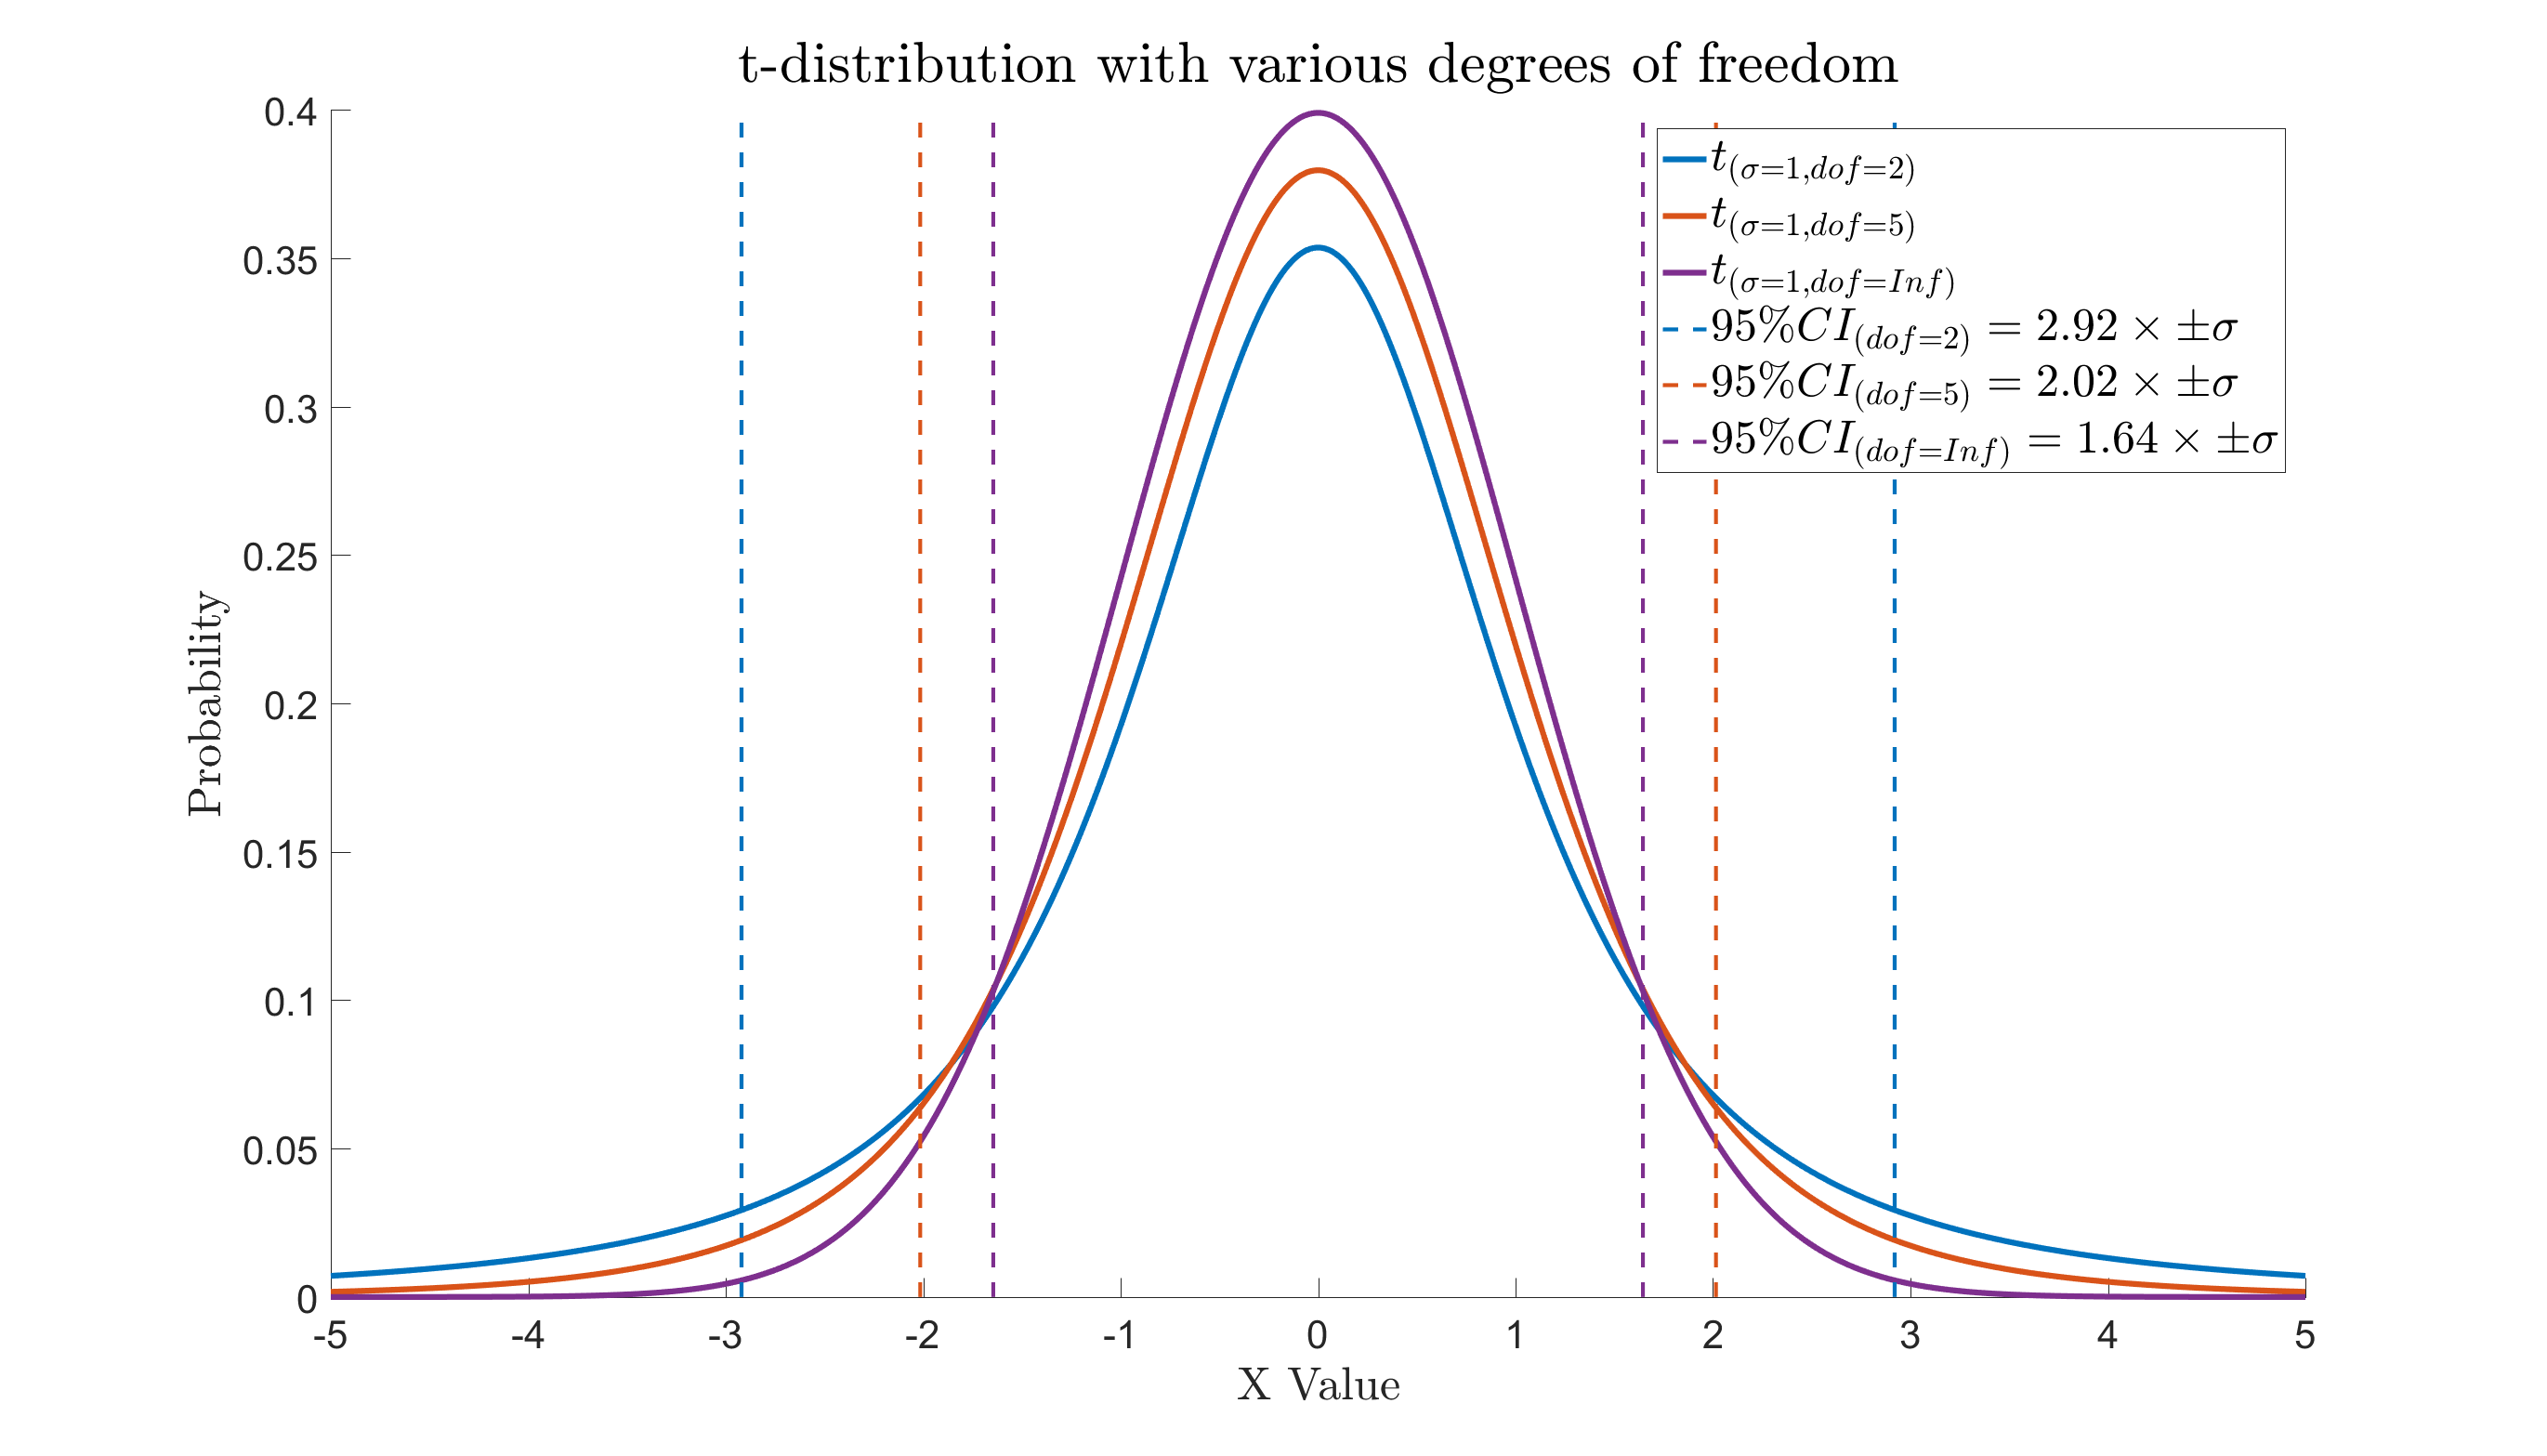
\includegraphics[height = 4in]{tdist.png}
\end{figure}

\subsection{2D Case (Error Rectangle)}